\documentclass{article}
\usepackage{amsmath}
\usepackage{color,pxfonts,fix-cm}
\usepackage{latexsym}
\usepackage[mathletters]{ucs}
\DeclareUnicodeCharacter{34}{\textquotedbl}
\DeclareUnicodeCharacter{46}{\textperiodcentered}
\DeclareUnicodeCharacter{8220}{\textquotedblleft}
\DeclareUnicodeCharacter{58}{$\colon$}
\DeclareUnicodeCharacter{8221}{\textquotedblright}
\DeclareUnicodeCharacter{8226}{$\bullet$}
\DeclareUnicodeCharacter{32}{$\ $}
\usepackage[T1]{fontenc}
\usepackage[utf8x]{inputenc}
\usepackage{pict2e}
\usepackage{wasysym}
\usepackage[english]{babel}
\usepackage{tikz}
\pagestyle{empty}
\usepackage[margin=0in,paperwidth=595pt,paperheight=841pt]{geometry}
\begin{document}
\definecolor{color_29791}{rgb}{0,0,0}
\definecolor{color_283006}{rgb}{1,1,1}
\begin{tikzpicture}[overlay]\path(0pt,0pt);\end{tikzpicture}
\begin{picture}(-5,0)(2.5,0)
\put(136.94,-84.97998){\fontsize{14.04}{1}\usefont{T1}{cmr}{m}{n}\selectfont\color{color_29791}UNIVERSIDAD NACIONAL DE INGENIERÍA  }
\put(196.25,-115.58){\fontsize{14.04}{1}\usefont{T1}{cmr}{m}{n}\selectfont\color{color_29791}FACULTAD DE CIENCIAS  }
\put(131.42,-135.14){\fontsize{14.04}{1}\usefont{T1}{cmr}{m}{n}\selectfont\color{color_29791}FUNDAMENTOS DE PROGRAMACION-CC112 }
\put(282.65,-150.98){\fontsize{9.96}{1}\usefont{T1}{cmr}{m}{n}\selectfont\color{color_29791} }
\put(352.39,-329.69){\fontsize{11.04}{1}\usefont{T1}{cmr}{m}{n}\selectfont\color{color_29791} }
\put(282.65,-342.05){\fontsize{11.04}{1}\usefont{T1}{cmr}{m}{n}\selectfont\color{color_29791} }
\put(119.18,-360.29){\fontsize{14.04}{1}\usefont{T1}{cmr}{m}{n}\selectfont\color{color_29791}ESCUELA DE PROFESIONAL DE CIENCIA DE LA }
\put(228.29,-377.69){\fontsize{14.04}{1}\usefont{T1}{cmr}{m}{n}\selectfont\color{color_29791}COMPUTACION }
\put(177.05,-396.05){\fontsize{14.04}{1}\usefont{T1}{cmr}{m}{n}\selectfont\color{color_29791}PROYECTO FINAL DEL CURSO }
\put(70.104,-440.47){\fontsize{14.04}{1}\usefont{T1}{cmr}{m}{n}\selectfont\color{color_29791}SECCIÓN: D                                    DÍA Y HORA: 28/06/24 1PM-3PM  }
\put(70.104,-476.95){\fontsize{12}{1}\usefont{T1}{cmr}{m}{n}\selectfont\color{color_29791}Apellidos y Nombres:                                                         Código:                         }
\put(70.104,-492.79){\fontsize{12}{1}\usefont{T1}{cmr}{m}{n}\selectfont\color{color_29791}  }
\end{picture}
\begin{tikzpicture}[overlay]
\path(0pt,0pt);
\begin{scope}
\clip
(71.064pt, -520.03pt) -- (347.594pt, -520.03pt)
 -- (347.594pt, -520.03pt)
 -- (347.594pt, -503.47pt)
 -- (347.594pt, -503.47pt)
 -- (71.064pt, -503.47pt) -- cycle
;
\filldraw[color_283006][even odd rule]
(75.624pt, -517.27pt) -- (257.564pt, -517.27pt)
 -- (257.564pt, -517.27pt)
 -- (257.564pt, -503.47pt)
 -- (257.564pt, -503.47pt)
 -- (75.624pt, -503.47pt) -- cycle
;
\begin{scope}
\clip
(71.064pt, -520.03pt) -- (347.594pt, -520.03pt)
 -- (347.594pt, -520.03pt)
 -- (347.594pt, -503.47pt)
 -- (347.594pt, -503.47pt)
 -- (71.064pt, -503.47pt) -- cycle
;
\end{scope}
\end{scope}
\end{tikzpicture}
\begin{picture}(-5,0)(2.5,0)
\put(75.624,-514.63){\fontsize{12}{1}\usefont{T1}{cmr}{m}{n}\selectfont\color{color_29791}Robles Urcia Miguel Angel Sebastian }
\end{picture}
\begin{tikzpicture}[overlay]
\path(0pt,0pt);
\begin{scope}
\clip
(348.67pt, -520.03pt) -- (519.45pt, -520.03pt)
 -- (519.45pt, -520.03pt)
 -- (519.45pt, -503.47pt)
 -- (519.45pt, -503.47pt)
 -- (348.67pt, -503.47pt) -- cycle
;
\filldraw[color_283006][even odd rule]
(353.11pt, -517.27pt) -- (407.83pt, -517.27pt)
 -- (407.83pt, -517.27pt)
 -- (407.83pt, -503.47pt)
 -- (407.83pt, -503.47pt)
 -- (353.11pt, -503.47pt) -- cycle
;
\begin{scope}
\clip
(348.67pt, -520.03pt) -- (519.45pt, -520.03pt)
 -- (519.45pt, -520.03pt)
 -- (519.45pt, -503.47pt)
 -- (519.45pt, -503.47pt)
 -- (348.67pt, -503.47pt) -- cycle
;
\end{scope}
\end{scope}
\end{tikzpicture}
\begin{picture}(-5,0)(2.5,0)
\put(353.11,-514.63){\fontsize{12}{1}\usefont{T1}{cmr}{m}{n}\selectfont\color{color_29791}20221608F }
\end{picture}
\begin{tikzpicture}[overlay]
\path(0pt,0pt);
\filldraw[color_283006][even odd rule]
(70.104pt, -503.47pt) -- (71.064pt, -503.47pt)
 -- (71.064pt, -503.47pt)
 -- (71.064pt, -497.47pt)
 -- (71.064pt, -497.47pt)
 -- (70.104pt, -497.47pt) -- cycle
;
\filldraw[color_283006][even odd rule]
(70.104pt, -498.43pt) -- (71.064pt, -498.43pt)
 -- (71.064pt, -498.43pt)
 -- (71.064pt, -497.47pt)
 -- (71.064pt, -497.47pt)
 -- (70.104pt, -497.47pt) -- cycle
;
\filldraw[color_283006][even odd rule]
(71.064pt, -498.43pt) -- (347.714pt, -498.43pt)
 -- (347.714pt, -498.43pt)
 -- (347.714pt, -497.47pt)
 -- (347.714pt, -497.47pt)
 -- (71.064pt, -497.47pt) -- cycle
;
\filldraw[color_283006][even odd rule]
(347.71pt, -503.47pt) -- (348.67pt, -503.47pt)
 -- (348.67pt, -503.47pt)
 -- (348.67pt, -498.43pt)
 -- (348.67pt, -498.43pt)
 -- (347.71pt, -498.43pt) -- cycle
;
\filldraw[color_283006][even odd rule]
(347.71pt, -498.43pt) -- (348.67pt, -498.43pt)
 -- (348.67pt, -498.43pt)
 -- (348.67pt, -497.47pt)
 -- (348.67pt, -497.47pt)
 -- (347.71pt, -497.47pt) -- cycle
;
\filldraw[color_283006][even odd rule]
(348.67pt, -498.43pt) -- (519.45pt, -498.43pt)
 -- (519.45pt, -498.43pt)
 -- (519.45pt, -497.47pt)
 -- (519.45pt, -497.47pt)
 -- (348.67pt, -497.47pt) -- cycle
;
\filldraw[color_283006][even odd rule]
(519.46pt, -503.47pt) -- (520.42pt, -503.47pt)
 -- (520.42pt, -503.47pt)
 -- (520.42pt, -497.47pt)
 -- (520.42pt, -497.47pt)
 -- (519.46pt, -497.47pt) -- cycle
;
\filldraw[color_283006][even odd rule]
(519.46pt, -498.43pt) -- (520.42pt, -498.43pt)
 -- (520.42pt, -498.43pt)
 -- (520.42pt, -497.47pt)
 -- (520.42pt, -497.47pt)
 -- (519.46pt, -497.47pt) -- cycle
;
\filldraw[color_283006][even odd rule]
(70.104pt, -524.95pt) -- (71.064pt, -524.95pt)
 -- (71.064pt, -524.95pt)
 -- (71.064pt, -503.47pt)
 -- (71.064pt, -503.47pt)
 -- (70.104pt, -503.47pt) -- cycle
;
\filldraw[color_283006][even odd rule]
(347.71pt, -524.95pt) -- (348.67pt, -524.95pt)
 -- (348.67pt, -524.95pt)
 -- (348.67pt, -503.47pt)
 -- (348.67pt, -503.47pt)
 -- (347.71pt, -503.47pt) -- cycle
;
\filldraw[color_283006][even odd rule]
(519.46pt, -524.95pt) -- (520.42pt, -524.95pt)
 -- (520.42pt, -524.95pt)
 -- (520.42pt, -503.47pt)
 -- (520.42pt, -503.47pt)
 -- (519.46pt, -503.47pt) -- cycle
;
\begin{scope}
\clip
(71.064pt, -547.51pt) -- (347.594pt, -547.51pt)
 -- (347.594pt, -547.51pt)
 -- (347.594pt, -530.95pt)
 -- (347.594pt, -530.95pt)
 -- (71.064pt, -530.95pt) -- cycle
;
\begin{scope}
\clip
(71.064pt, -547.51pt) -- (347.594pt, -547.51pt)
 -- (347.594pt, -547.51pt)
 -- (347.594pt, -530.95pt)
 -- (347.594pt, -530.95pt)
 -- (71.064pt, -530.95pt) -- cycle
;
\end{scope}
\end{scope}
\end{tikzpicture}
\begin{picture}(-5,0)(2.5,0)
\put(75.624,-542.11){\fontsize{12}{1}\usefont{T1}{cmr}{m}{n}\selectfont\color{color_29791}  }
\end{picture}
\begin{tikzpicture}[overlay]
\path(0pt,0pt);
\filldraw[color_283006][even odd rule]
(70.104pt, -530.95pt) -- (71.064pt, -530.95pt)
 -- (71.064pt, -530.95pt)
 -- (71.064pt, -524.95pt)
 -- (71.064pt, -524.95pt)
 -- (70.104pt, -524.95pt) -- cycle
;
\filldraw[color_283006][even odd rule]
(71.064pt, -525.91pt) -- (347.714pt, -525.91pt)
 -- (347.714pt, -525.91pt)
 -- (347.714pt, -524.95pt)
 -- (347.714pt, -524.95pt)
 -- (71.064pt, -524.95pt) -- cycle
;
\filldraw[color_283006][even odd rule]
(347.71pt, -530.95pt) -- (348.67pt, -530.95pt)
 -- (348.67pt, -530.95pt)
 -- (348.67pt, -524.95pt)
 -- (348.67pt, -524.95pt)
 -- (347.71pt, -524.95pt) -- cycle
;
\filldraw[color_283006][even odd rule]
(348.67pt, -525.91pt) -- (519.45pt, -525.91pt)
 -- (519.45pt, -525.91pt)
 -- (519.45pt, -524.95pt)
 -- (519.45pt, -524.95pt)
 -- (348.67pt, -524.95pt) -- cycle
;
\filldraw[color_283006][even odd rule]
(519.46pt, -530.95pt) -- (520.42pt, -530.95pt)
 -- (520.42pt, -530.95pt)
 -- (520.42pt, -524.95pt)
 -- (520.42pt, -524.95pt)
 -- (519.46pt, -524.95pt) -- cycle
;
\filldraw[color_283006][even odd rule]
(70.104pt, -552.55pt) -- (71.064pt, -552.55pt)
 -- (71.064pt, -552.55pt)
 -- (71.064pt, -530.95pt)
 -- (71.064pt, -530.95pt)
 -- (70.104pt, -530.95pt) -- cycle
;
\filldraw[color_283006][even odd rule]
(347.71pt, -552.55pt) -- (348.67pt, -552.55pt)
 -- (348.67pt, -552.55pt)
 -- (348.67pt, -530.95pt)
 -- (348.67pt, -530.95pt)
 -- (347.71pt, -530.95pt) -- cycle
;
\filldraw[color_283006][even odd rule]
(519.46pt, -552.55pt) -- (520.42pt, -552.55pt)
 -- (520.42pt, -552.55pt)
 -- (520.42pt, -530.95pt)
 -- (520.42pt, -530.95pt)
 -- (519.46pt, -530.95pt) -- cycle
;
\begin{scope}
\clip
(71.064pt, -574.99pt) -- (347.594pt, -574.99pt)
 -- (347.594pt, -574.99pt)
 -- (347.594pt, -558.55pt)
 -- (347.594pt, -558.55pt)
 -- (71.064pt, -558.55pt) -- cycle
;
\begin{scope}
\clip
(71.064pt, -574.99pt) -- (347.594pt, -574.99pt)
 -- (347.594pt, -574.99pt)
 -- (347.594pt, -558.55pt)
 -- (347.594pt, -558.55pt)
 -- (71.064pt, -558.55pt) -- cycle
;
\end{scope}
\end{scope}
\end{tikzpicture}
\begin{picture}(-5,0)(2.5,0)
\put(75.624,-569.71){\fontsize{12}{1}\usefont{T1}{cmr}{m}{n}\selectfont\color{color_29791}Camarena Frías Ricardo David 20221526J }
\end{picture}
\begin{tikzpicture}[overlay]
\path(0pt,0pt);
\filldraw[color_283006][even odd rule]
(70.104pt, -558.55pt) -- (71.064pt, -558.55pt)
 -- (71.064pt, -558.55pt)
 -- (71.064pt, -552.55pt)
 -- (71.064pt, -552.55pt)
 -- (70.104pt, -552.55pt) -- cycle
;
\filldraw[color_283006][even odd rule]
(71.064pt, -553.51pt) -- (347.714pt, -553.51pt)
 -- (347.714pt, -553.51pt)
 -- (347.714pt, -552.55pt)
 -- (347.714pt, -552.55pt)
 -- (71.064pt, -552.55pt) -- cycle
;
\filldraw[color_283006][even odd rule]
(347.71pt, -558.55pt) -- (348.67pt, -558.55pt)
 -- (348.67pt, -558.55pt)
 -- (348.67pt, -552.55pt)
 -- (348.67pt, -552.55pt)
 -- (347.71pt, -552.55pt) -- cycle
;
\filldraw[color_283006][even odd rule]
(348.67pt, -553.51pt) -- (519.45pt, -553.51pt)
 -- (519.45pt, -553.51pt)
 -- (519.45pt, -552.55pt)
 -- (519.45pt, -552.55pt)
 -- (348.67pt, -552.55pt) -- cycle
;
\filldraw[color_283006][even odd rule]
(519.46pt, -558.55pt) -- (520.42pt, -558.55pt)
 -- (520.42pt, -558.55pt)
 -- (520.42pt, -552.55pt)
 -- (520.42pt, -552.55pt)
 -- (519.46pt, -552.55pt) -- cycle
;
\filldraw[color_283006][even odd rule]
(70.104pt, -580.03pt) -- (71.064pt, -580.03pt)
 -- (71.064pt, -580.03pt)
 -- (71.064pt, -558.55pt)
 -- (71.064pt, -558.55pt)
 -- (70.104pt, -558.55pt) -- cycle
;
\filldraw[color_283006][even odd rule]
(70.104pt, -580.99pt) -- (71.064pt, -580.99pt)
 -- (71.064pt, -580.99pt)
 -- (71.064pt, -580.03pt)
 -- (71.064pt, -580.03pt)
 -- (70.104pt, -580.03pt) -- cycle
;
\filldraw[color_283006][even odd rule]
(70.104pt, -580.99pt) -- (71.064pt, -580.99pt)
 -- (71.064pt, -580.99pt)
 -- (71.064pt, -580.03pt)
 -- (71.064pt, -580.03pt)
 -- (70.104pt, -580.03pt) -- cycle
;
\filldraw[color_283006][even odd rule]
(71.064pt, -580.99pt) -- (347.714pt, -580.99pt)
 -- (347.714pt, -580.99pt)
 -- (347.714pt, -580.03pt)
 -- (347.714pt, -580.03pt)
 -- (71.064pt, -580.03pt) -- cycle
;
\filldraw[color_283006][even odd rule]
(347.71pt, -580.03pt) -- (348.67pt, -580.03pt)
 -- (348.67pt, -580.03pt)
 -- (348.67pt, -558.55pt)
 -- (348.67pt, -558.55pt)
 -- (347.71pt, -558.55pt) -- cycle
;
\filldraw[color_283006][even odd rule]
(347.71pt, -580.99pt) -- (348.67pt, -580.99pt)
 -- (348.67pt, -580.99pt)
 -- (348.67pt, -580.03pt)
 -- (348.67pt, -580.03pt)
 -- (347.71pt, -580.03pt) -- cycle
;
\filldraw[color_283006][even odd rule]
(348.67pt, -580.99pt) -- (519.45pt, -580.99pt)
 -- (519.45pt, -580.99pt)
 -- (519.45pt, -580.03pt)
 -- (519.45pt, -580.03pt)
 -- (348.67pt, -580.03pt) -- cycle
;
\filldraw[color_283006][even odd rule]
(519.46pt, -580.03pt) -- (520.42pt, -580.03pt)
 -- (520.42pt, -580.03pt)
 -- (520.42pt, -558.55pt)
 -- (520.42pt, -558.55pt)
 -- (519.46pt, -558.55pt) -- cycle
;
\filldraw[color_283006][even odd rule]
(519.46pt, -580.99pt) -- (520.42pt, -580.99pt)
 -- (520.42pt, -580.99pt)
 -- (520.42pt, -580.03pt)
 -- (520.42pt, -580.03pt)
 -- (519.46pt, -580.03pt) -- cycle
;
\filldraw[color_283006][even odd rule]
(519.46pt, -580.99pt) -- (520.42pt, -580.99pt)
 -- (520.42pt, -580.99pt)
 -- (520.42pt, -580.03pt)
 -- (520.42pt, -580.03pt)
 -- (519.46pt, -580.03pt) -- cycle
;
\end{tikzpicture}
\begin{picture}(-5,0)(2.5,0)
\put(70.104,-604.15){\fontsize{12}{1}\usefont{T1}{cmr}{m}{n}\selectfont\color{color_29791}Nombres de los Docentes:  }
\put(70.104,-632.02){\fontsize{12}{1}\usefont{T1}{cmr}{m}{n}\selectfont\color{color_29791}- Americo Andres Chulluncuy Reynoso }
\put(70.104,-649.06){\fontsize{12}{1}\usefont{T1}{cmr}{m}{n}\selectfont\color{color_29791} }
\put(70.104,-664.78){\fontsize{12}{1}\usefont{T1}{cmr}{m}{n}\selectfont\color{color_29791} }
\put(70.104,-690.58){\fontsize{14.04}{1}\usefont{T1}{cmr}{m}{n}\selectfont\color{color_29791}Fecha de entrega del informe: 28/06/24 }
\put(254.33,-733.656){\fontsize{20.04}{1}\usefont{T1}{cmr}{m}{n}\selectfont\color{color_29791}2024-1 }
\put(70.104,-752.736){\fontsize{12}{1}\usefont{T1}{cmr}{m}{n}\selectfont\color{color_29791} }
\put(212.9,-329.64){
\includegraphics[width=139.5pt,height=174pt]{latexImage_c5a7afbada58bdb148deb446dff63715.png}}
\end{picture}
\newpage
\begin{tikzpicture}[overlay]\path(0pt,0pt);\end{tikzpicture}
\begin{picture}(-5,0)(2.5,0)
\put(70.104,-71.15997){\fontsize{12}{1}\usefont{T1}{cmr}{m}{n}\selectfont\color{color_29791} }
\put(88.1,-101.54){\fontsize{18}{1}\usefont{T1}{cmr}{m}{n}\selectfont\color{color_29791}1. Introducción }
\put(70.104,-127.7){\fontsize{12}{1}\usefont{T1}{cmr}{m}{n}\selectfont\color{color_29791}En este informe detallamos el desarrollo de nuestros ejercicios explicando la relación de }
\put(70.104,-143.66){\fontsize{12}{1}\usefont{T1}{cmr}{m}{n}\selectfont\color{color_29791}las ideas hasta la codificación, también exponemos el fundamento teórico utilizado y las }
\put(70.104,-159.5){\fontsize{12}{1}\usefont{T1}{cmr}{m}{n}\selectfont\color{color_29791}conclusiones }
\put(70.104,-183.38){\fontsize{12}{1}\usefont{T1}{cmr}{m}{n}\selectfont\color{color_29791} }
\put(106.1,-207.26){\fontsize{12}{1}\usefont{T1}{cmr}{m}{n}\selectfont\color{color_29791} }
\put(88.1,-228.74){\fontsize{18}{1}\usefont{T1}{cmr}{m}{n}\selectfont\color{color_29791}2. Fundamento teórico }
\put(106.1,-246.86){\fontsize{12}{1}\usefont{T1}{cmr}{m}{n}\selectfont\color{color_29791} }
\put(106.1,-261.77){\fontsize{12}{1}\usefont{T1}{cmr}{m}{n}\selectfont\color{color_29791}Funciones: }
\put(106.1,-277.73){\fontsize{12}{1}\usefont{T1}{cmr}{m}{n}\selectfont\color{color_29791}Es un código o sentencias, consta del nombre de la función y los parámetros }
\put(106.1,-293.57){\fontsize{12}{1}\usefont{T1}{cmr}{m}{n}\selectfont\color{color_29791}separados por comas.  }
\put(106.1,-308.57){\fontsize{11.04}{1}\usefont{T1}{cmr}{m}{n}\selectfont\color{color_29791} }
\put(487.18,-600.31){\fontsize{11.04}{1}\usefont{T1}{cmr}{m}{n}\selectfont\color{color_29791} }
\put(106.1,-612.58){\fontsize{11.04}{1}\usefont{T1}{cmr}{m}{n}\selectfont\color{color_29791} }
\put(106.1,-628.9){\fontsize{12}{1}\usefont{T1}{cmr}{m}{n}\selectfont\color{color_29791}Cadenas: }
\put(106.1,-644.74){\fontsize{12}{1}\usefont{T1}{cmr}{m}{n}\selectfont\color{color_29791}Son una secuencia de caracteres se pueden crear utilizando comillas simples o }
\put(106.1,-660.58){\fontsize{12}{1}\usefont{T1}{cmr}{m}{n}\selectfont\color{color_29791}dobles  }
\put(106.1,-674.74){\fontsize{9.96}{1}\usefont{T1}{cmr}{m}{n}\selectfont\color{color_29791} }
\put(106.1,-689.74){\fontsize{12}{1}\usefont{T1}{cmr}{m}{n}\selectfont\color{color_29791}Listas: }
\put(106.1,-705.58){\fontsize{12}{1}\usefont{T1}{cmr}{m}{n}\selectfont\color{color_29791}Las listas en python se crean usando corchetes [] y pueden contener datos como }
\put(106.1,-721.42){\fontsize{12}{1}\usefont{T1}{cmr}{m}{n}\selectfont\color{color_29791}enteros, flotantes o cadenas. Las listas en python son dinámicas porque pueden }
\put(106.1,-737.256){\fontsize{12}{1}\usefont{T1}{cmr}{m}{n}\selectfont\color{color_29791}cambiar de tamaño en cualquier momento también son ordenadas y se accede }
\put(106.1,-753.216){\fontsize{12}{1}\usefont{T1}{cmr}{m}{n}\selectfont\color{color_29791}media}
\put(106.05,-599.41){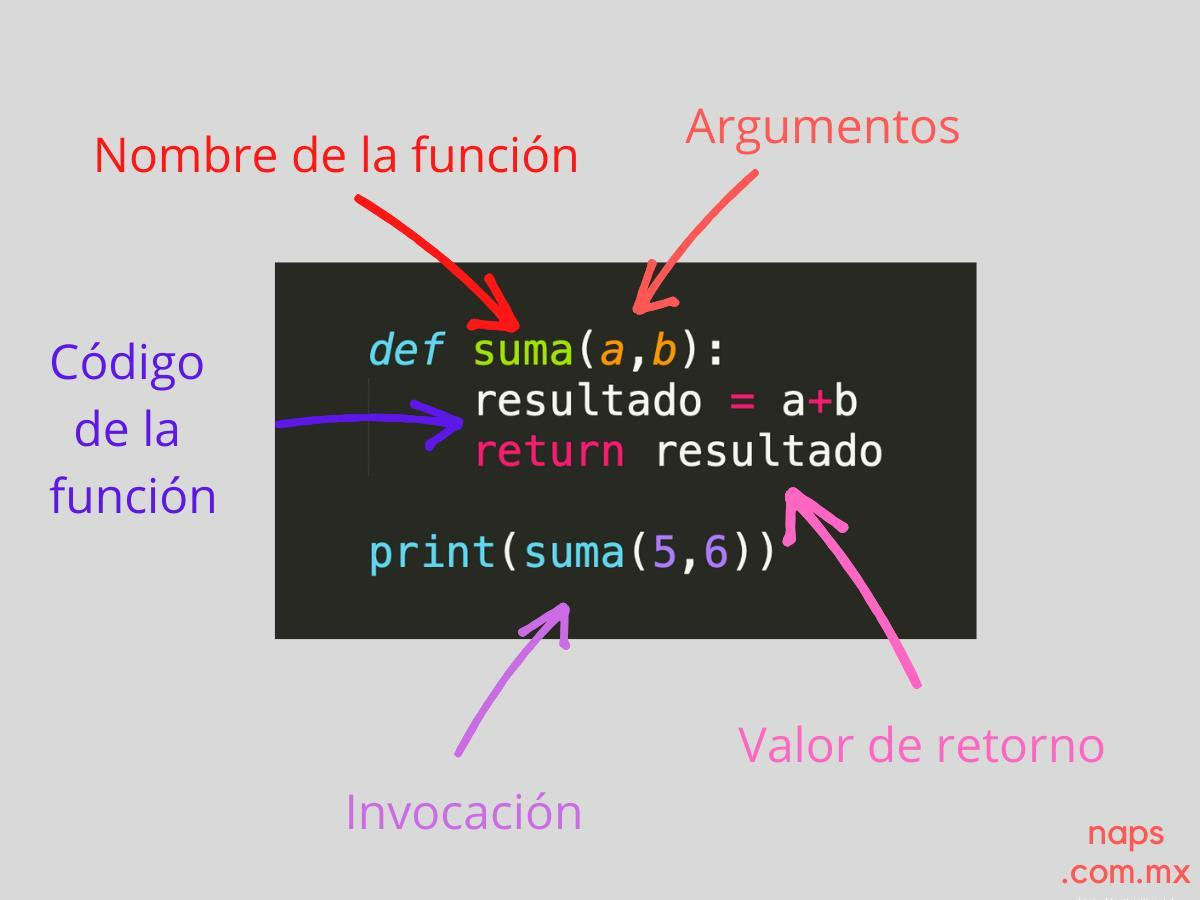
\includegraphics[width=380.94pt,height=285.75pt]{latexImage_8adbf84e82f67d392179ab85ff668a37.png}}
\end{picture}
\newpage
\begin{tikzpicture}[overlay]\path(0pt,0pt);\end{tikzpicture}
\begin{picture}(-5,0)(2.5,0)
\put(106.1,-70.20001){\fontsize{11.04}{1}\usefont{T1}{cmr}{m}{n}\selectfont\color{color_29791} }
\put(470.62,-302.09){\fontsize{11.04}{1}\usefont{T1}{cmr}{m}{n}\selectfont\color{color_29791} }
\put(106.1,-314.45){\fontsize{11.04}{1}\usefont{T1}{cmr}{m}{n}\selectfont\color{color_29791} }
\put(106.1,-331.73){\fontsize{12.96}{1}\usefont{T1}{cmr}{b}{n}\selectfont\color{color_29791}Diccionarios: }
\put(106.1,-349.97){\fontsize{12.96}{1}\usefont{T1}{cmr}{m}{n}\selectfont\color{color_29791}Son estructuras que almacenan pares de clave-valor generalmente }
\put(106.1,-368.21){\fontsize{12.96}{1}\usefont{T1}{cmr}{m}{n}\selectfont\color{color_29791}son datos que tienen una relación lógica. Se crean usando llaves \{\}, }
\put(106.1,-386.57){\fontsize{12.96}{1}\usefont{T1}{cmr}{m}{n}\selectfont\color{color_29791}algunas características es que se pueden añadir mas elementos }
\put(106.1,-404.81){\fontsize{12.96}{1}\usefont{T1}{cmr}{m}{n}\selectfont\color{color_29791}luego de ser creado  }
\put(106.1,-421.13){\fontsize{11.04}{1}\usefont{T1}{cmr}{m}{n}\selectfont\color{color_29791} }
\put(467.62,-615.22){\fontsize{11.04}{1}\usefont{T1}{cmr}{m}{n}\selectfont\color{color_29791} }
\put(106.1,-627.58){\fontsize{11.04}{1}\usefont{T1}{cmr}{m}{n}\selectfont\color{color_29791} }
\put(106.1,-644.98){\fontsize{12.96}{1}\usefont{T1}{cmr}{b}{n}\selectfont\color{color_29791}Clases: }
\put(106.1,-663.22){\fontsize{12.96}{1}\usefont{T1}{cmr}{m}{n}\selectfont\color{color_29791}Para crear una clase se utiliza class seguidamente el nombre de la }
\put(106.1,-681.46){\fontsize{12.96}{1}\usefont{T1}{cmr}{m}{n}\selectfont\color{color_29791}clase y dos puntos. }
\put(106.1,-698.62){\fontsize{12}{1}\usefont{T1}{cmr}{m}{n}\selectfont\color{color_29791} }
\put(106.1,-713.5){\fontsize{12}{1}\usefont{T1}{cmr}{m}{n}\selectfont\color{color_29791} }
\put(106.1,-729.34){\fontsize{12}{1}\usefont{T1}{cmr}{m}{n}\selectfont\color{color_29791} }
\put(88.1,-750.936){\fontsize{18}{1}\usefont{T1}{cmr}{m}{n}\selectfont\color{color_29791}3.}
\put(106.05,-302.02){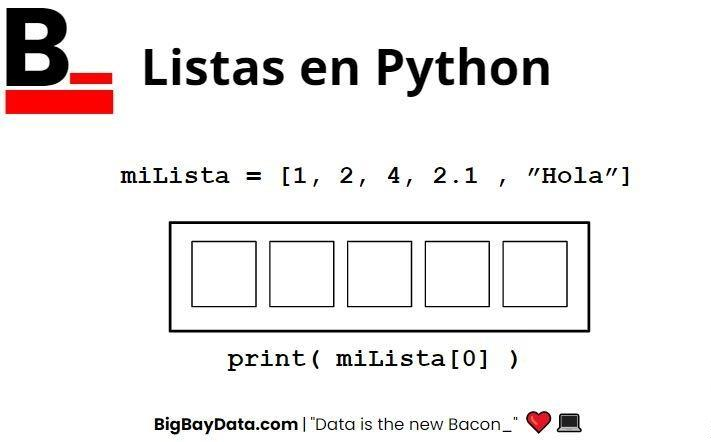
\includegraphics[width=364.35pt,height=226.65pt]{latexImage_5158bc5379d4918f30ae42050b50b940.png}}
\put(106.05,-614.82){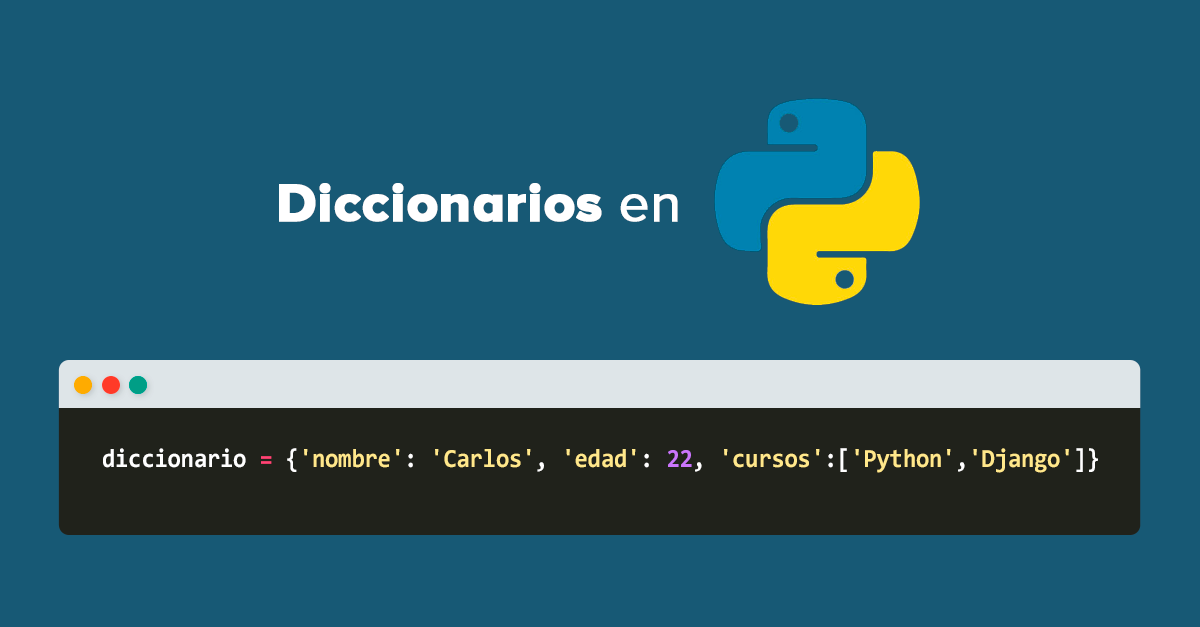
\includegraphics[width=361.08pt,height=188.65pt]{latexImage_162435e479737c7cdde60a118393efa3.png}}
\end{picture}
\newpage
\begin{tikzpicture}[overlay]\path(0pt,0pt);\end{tikzpicture}
\begin{picture}(-5,0)(2.5,0)
\put(106.1,-71.03998){\fontsize{12}{1}\usefont{T1}{cmr}{m}{n}\selectfont\color{color_29791} }
\put(106.1,-87.97998){\fontsize{12}{1}\usefont{T1}{cmr}{m}{n}\selectfont\color{color_29791}• Parte1 }
\put(124.1,-103.7){\fontsize{12}{1}\usefont{T1}{cmr}{m}{n}\selectfont\color{color_29791}Ejercicio 1(Funciones): }
\put(124.1,-127.58){\fontsize{12}{1}\usefont{T1}{cmr}{m}{n}\selectfont\color{color_29791}Primero definimos una función llamada “Factorial” para cualquier n (entero }
\put(124.1,-143.42){\fontsize{12}{1}\usefont{T1}{cmr}{m}{n}\selectfont\color{color_29791}no negativo) si el numero n ingresado es negativo, el programa te volverá a }
\put(124.1,-159.26){\fontsize{12}{1}\usefont{T1}{cmr}{m}{n}\selectfont\color{color_29791}pedir que digites un numero valido. }
\put(124.1,-183.14){\fontsize{12}{1}\usefont{T1}{cmr}{m}{n}\selectfont\color{color_29791}Luego viene el caso Base, donde si el numero ingresado es 0 o 1, el factorial }
\put(124.1,-199.1){\fontsize{12}{1}\usefont{T1}{cmr}{m}{n}\selectfont\color{color_29791}me dará 1. }
\put(124.1,-222.98){\fontsize{12}{1}\usefont{T1}{cmr}{m}{n}\selectfont\color{color_29791}El cálculo iterativo si n es mayor que 1, inicializa "resultado” en 1, con el }
\put(124.1,-238.82){\fontsize{12}{1}\usefont{T1}{cmr}{m}{n}\selectfont\color{color_29791}bucle itera desde 2 hasta n, seguido de multiplicar "resultado” por el valor }
\put(124.1,-254.69){\fontsize{12}{1}\usefont{T1}{cmr}{m}{n}\selectfont\color{color_29791}actual de i en cada iteración a continuación, retorna el valor de "resultado” }
\put(124.1,-270.53){\fontsize{12}{1}\usefont{T1}{cmr}{m}{n}\selectfont\color{color_29791}que es el factorial de n }
\put(505.66,-505.27){\fontsize{12}{1}\usefont{T1}{cmr}{m}{n}\selectfont\color{color_29791} }
\put(124.1,-526.51){\fontsize{12}{1}\usefont{T1}{cmr}{m}{n}\selectfont\color{color_29791}Finalmente tenemos el bucle while para la entrada del usuario. }
\put(495.22,-701.62){\fontsize{12}{1}\usefont{T1}{cmr}{m}{n}\selectfont\color{color_29791} }
\put(124.1,-722.14){\fontsize{11.04}{1}\usefont{T1}{cmr}{m}{n}\selectfont\color{color_29791}E}
\put(124.05,-505.22){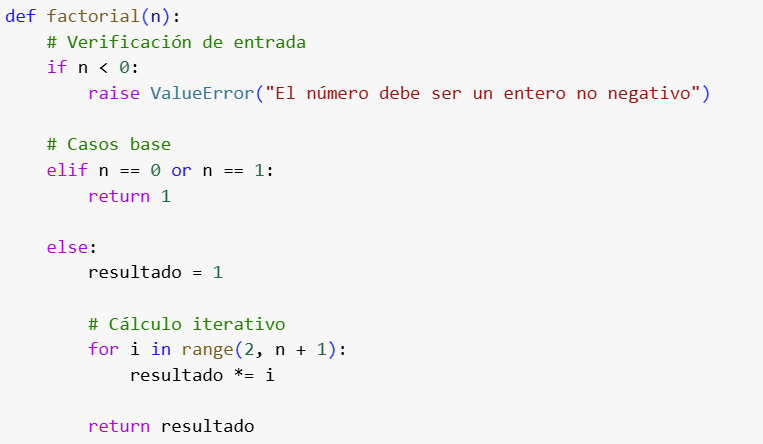
\includegraphics[width=381.5pt,height=222pt]{latexImage_e2aa24cb5d7a14a8d265f1dac4139a77.png}}
\put(124.05,-701.6){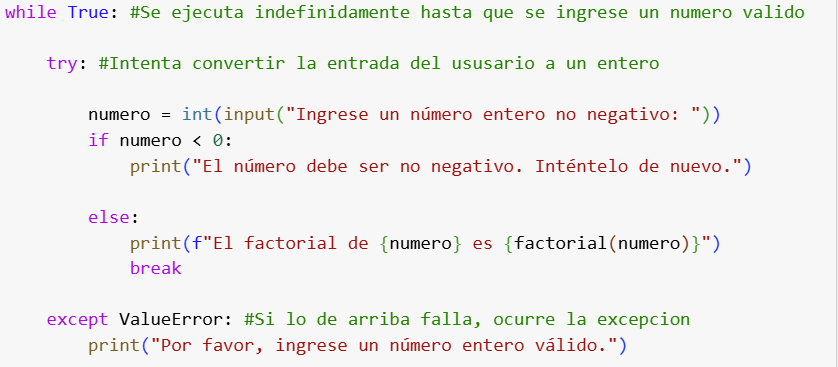
\includegraphics[width=371.05pt,height=162.5pt]{latexImage_488a86c5e84d9763a4c649732d165856.png}}
\end{picture}
\newpage
\begin{tikzpicture}[overlay]\path(0pt,0pt);\end{tikzpicture}
\begin{picture}(-5,0)(2.5,0)
\put(124.1,-71.03998){\fontsize{12}{1}\usefont{T1}{cmr}{m}{n}\selectfont\color{color_29791}Definimos una función llamada “invertir\_cadena”, esta función toma un }
\put(124.1,-87.02002){\fontsize{12}{1}\usefont{T1}{cmr}{m}{n}\selectfont\color{color_29791}parámetro llamado “cadena” que es el texto que se desea invertir. }
\put(124.1,-110.9){\fontsize{12}{1}\usefont{T1}{cmr}{m}{n}\selectfont\color{color_29791}Se inicializa la variable “cadena\_invertida” como una cadena vacia donde se }
\put(124.1,-126.74){\fontsize{12}{1}\usefont{T1}{cmr}{m}{n}\selectfont\color{color_29791}almacenará la cadena invertida, el bucle for recorre cada carácter en la }
\put(124.1,-142.58){\fontsize{12}{1}\usefont{T1}{cmr}{m}{n}\selectfont\color{color_29791}cadena “cadena”. }
\put(124.1,-166.46){\fontsize{12}{1}\usefont{T1}{cmr}{m}{n}\selectfont\color{color_29791}En cada iteracion del bucle, el “carácter” actual se agrega al inicio de de la }
\put(124.1,-182.3){\fontsize{12}{1}\usefont{T1}{cmr}{m}{n}\selectfont\color{color_29791}cadena "cadena\_invertida”. }
\put(124.1,-206.18){\fontsize{12}{1}\usefont{T1}{cmr}{m}{n}\selectfont\color{color_29791}Una vez completado el bucle se retorna "cadena\_invertida” que contiene la }
\put(124.1,-222.02){\fontsize{12}{1}\usefont{T1}{cmr}{m}{n}\selectfont\color{color_29791}cadena original invertida. }
\put(124.1,-245.9){\fontsize{12}{1}\usefont{T1}{cmr}{m}{n}\selectfont\color{color_29791}Se utiliza input para pedirle al usuario que ingrese un texto, dicho texto se }
\put(124.1,-261.77){\fontsize{12}{1}\usefont{T1}{cmr}{m}{n}\selectfont\color{color_29791}guarda en la variable "cadena”. }
\put(124.1,-285.65){\fontsize{12}{1}\usefont{T1}{cmr}{m}{n}\selectfont\color{color_29791}Finalmente, print llama a la funcion “invertir\_cadena” con “cadena” como }
\put(124.1,-301.61){\fontsize{12}{1}\usefont{T1}{cmr}{m}{n}\selectfont\color{color_29791}argumento para obtener la cadena invertida. }
\put(549.36,-404.33){\fontsize{11.04}{1}\usefont{T1}{cmr}{m}{n}\selectfont\color{color_29791} }
\put(124.1,-424.49){\fontsize{11.04}{1}\usefont{T1}{cmr}{m}{n}\selectfont\color{color_29791} }
\put(124.1,-447.07){\fontsize{11.04}{1}\usefont{T1}{cmr}{m}{n}\selectfont\color{color_29791}Ejercicio 3: }
\put(124.1,-470.47){\fontsize{12}{1}\usefont{T1}{cmr}{m}{n}\selectfont\color{color_29791}Definimos una funcion “agregar\_elementos”, se inicializa una lista vacia }
\put(124.1,-486.31){\fontsize{12}{1}\usefont{T1}{cmr}{m}{n}\selectfont\color{color_29791}donde se almacenarán los elementos ingresados por el usuario. }
\put(124.1,-510.19){\fontsize{12}{1}\usefont{T1}{cmr}{m}{n}\selectfont\color{color_29791}Creamos un bucle “while” el cual se ejecutará indefinidamente, hasta que se }
\put(124.1,-526.03){\fontsize{12}{1}\usefont{T1}{cmr}{m}{n}\selectfont\color{color_29791}ejecute "break”, luego con el input solicita al usuario que ingrese un }
\put(124.1,-541.87){\fontsize{12}{1}\usefont{T1}{cmr}{m}{n}\selectfont\color{color_29791}elemento para agregar a la lista. }
\put(124.1,-565.75){\fontsize{12}{1}\usefont{T1}{cmr}{m}{n}\selectfont\color{color_29791}Con “elemento.lower()” verifica si el usuario ingreso la palabra “salir”, si el }
\put(124.1,-581.71){\fontsize{12}{1}\usefont{T1}{cmr}{m}{n}\selectfont\color{color_29791}usuario decide salir el bucle "while” se interrumpe. }
\put(124.1,-605.47){\fontsize{12}{1}\usefont{T1}{cmr}{m}{n}\selectfont\color{color_29791}Con “lista,append(elemento)” agrega el elemento ingresado por el usuario a }
\put(124.1,-621.46){\fontsize{12}{1}\usefont{T1}{cmr}{m}{n}\selectfont\color{color_29791}la lista }
\put(124.1,-645.34){\fontsize{12}{1}\usefont{T1}{cmr}{m}{n}\selectfont\color{color_29791}Luego con “print(f"Elemento '\{elemento\}' agregado. Lista actual: \{lista\}")” }
\put(124.1,-661.18){\fontsize{12}{1}\usefont{T1}{cmr}{m}{n}\selectfont\color{color_29791}imprime un mensaje confirmando que el elemento fue ingresado a la lista. }
\put(124.1,-685.06){\fontsize{12}{1}\usefont{T1}{cmr}{m}{n}\selectfont\color{color_29791}Finalmente, con el "return\_lista” la funcion retorna la lista completa con }
\put(124.1,-700.9){\fontsize{12}{1}\usefont{T1}{cmr}{m}{n}\selectfont\color{color_29791}todos}
\put(124.05,-403.87){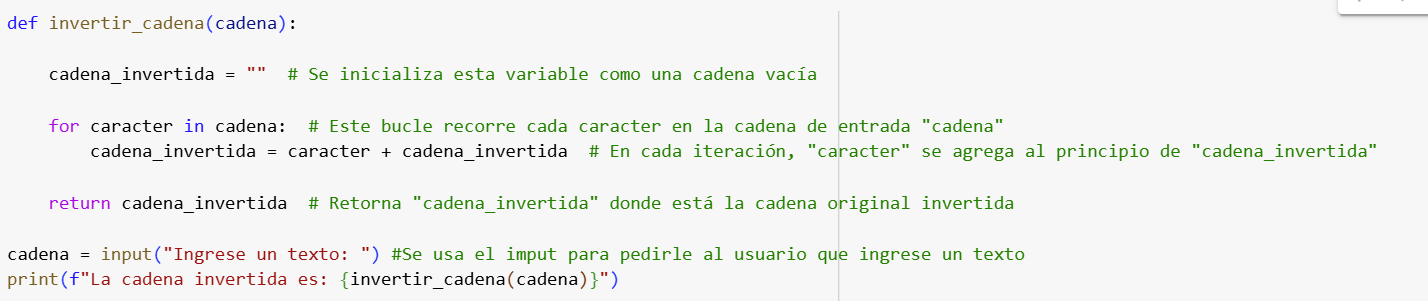
\includegraphics[width=425.2pt,height=89.65pt]{latexImage_ce8b57c7c8350c193e8ebfdd04a156c6.png}}
\end{picture}
\newpage
\begin{tikzpicture}[overlay]\path(0pt,0pt);\end{tikzpicture}
\begin{picture}(-5,0)(2.5,0)
\put(549.36,-192.26){\fontsize{11.04}{1}\usefont{T1}{cmr}{m}{n}\selectfont\color{color_29791} }
\put(70.104,-212.54){\fontsize{11.04}{1}\usefont{T1}{cmr}{m}{n}\selectfont\color{color_29791} }
\put(124.1,-235.1){\fontsize{11.04}{1}\usefont{T1}{cmr}{m}{n}\selectfont\color{color_29791}Ejercicio 4(Diccionarios): }
\put(124.1,-249.62){\fontsize{11.04}{1}\usefont{T1}{cmr}{m}{n}\selectfont\color{color_29791} }
\put(124.1,-266.09){\fontsize{12.96}{1}\usefont{T1}{cmr}{m}{n}\selectfont\color{color_29791}Primero queríamos crear un menú que muestre al usuario 5 opciones }
\put(124.1,-283.25){\fontsize{12.96}{1}\usefont{T1}{cmr}{m}{n}\selectfont\color{color_29791}para eso simplemente creamos una función que imprima las opciones }
\put(124.1,-300.41){\fontsize{12.96}{1}\usefont{T1}{cmr}{m}{n}\selectfont\color{color_29791} }
\put(422.62,-427.01){\fontsize{12.96}{1}\usefont{T1}{cmr}{m}{n}\selectfont\color{color_29791} }
\put(124.1,-441.19){\fontsize{12.96}{1}\usefont{T1}{cmr}{m}{n}\selectfont\color{color_29791} }
\put(124.1,-458.35){\fontsize{12.96}{1}\usefont{T1}{cmr}{m}{n}\selectfont\color{color_29791}Luego creamos un bucle while para que nos muestre las opciones }
\put(124.1,-475.51){\fontsize{12.96}{1}\usefont{T1}{cmr}{m}{n}\selectfont\color{color_29791}repetidamente, también usamos if else para indicar que hacer si se }
\put(124.1,-492.79){\fontsize{12.96}{1}\usefont{T1}{cmr}{m}{n}\selectfont\color{color_29791}selecciona una de las opciones }
\put(124.1,-509.95){\fontsize{12.96}{1}\usefont{T1}{cmr}{m}{n}\selectfont\color{color_29791} }
\put(124.05,-192.23){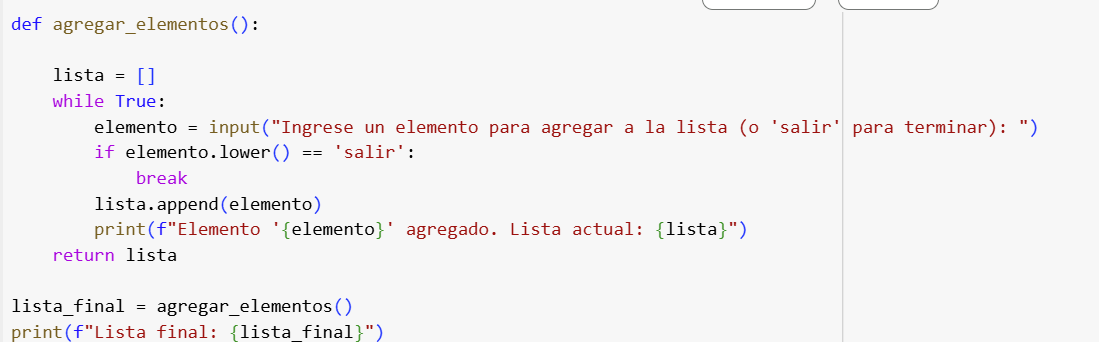
\includegraphics[width=425.2pt,height=132.3pt]{latexImage_9f4eba03c99bedb639f48c4511b82814.png}}
\put(124.05,-426.96){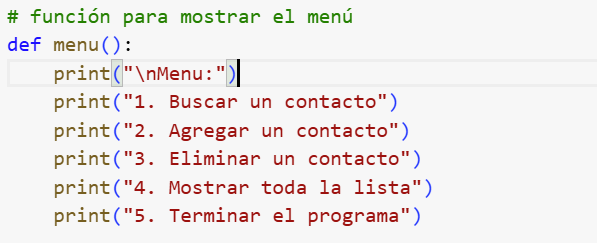
\includegraphics[width=298.5pt,height=121.5pt]{latexImage_c0416786362cccf28d41fb5764826b6e.png}}
\end{picture}
\newpage
\begin{tikzpicture}[overlay]\path(0pt,0pt);\end{tikzpicture}
\begin{picture}(-5,0)(2.5,0)
\put(549.36,-354.41){\fontsize{12.96}{1}\usefont{T1}{cmr}{m}{n}\selectfont\color{color_29791} }
\put(124.1,-368.81){\fontsize{12.96}{1}\usefont{T1}{cmr}{m}{n}\selectfont\color{color_29791} }
\put(124.1,-385.13){\fontsize{12}{1}\usefont{T1}{cmr}{m}{n}\selectfont\color{color_29791}Luego creamos un diccionario vacío }
\put(124.1,-401.93){\fontsize{12.96}{1}\usefont{T1}{cmr}{m}{n}\selectfont\color{color_29791} }
\put(311.59,-439.99){\fontsize{12.96}{1}\usefont{T1}{cmr}{m}{n}\selectfont\color{color_29791} }
\put(124.1,-454.39){\fontsize{12.96}{1}\usefont{T1}{cmr}{m}{n}\selectfont\color{color_29791} }
\put(124.1,-470.59){\fontsize{12}{1}\usefont{T1}{cmr}{m}{n}\selectfont\color{color_29791}Luego definimos las funciones que usaremos para cada opción }
\put(124.1,-487.39){\fontsize{12.96}{1}\usefont{T1}{cmr}{m}{n}\selectfont\color{color_29791} }
\put(476.62,-730.06){\fontsize{12.96}{1}\usefont{T1}{cmr}{m}{n}\selectfont\color{color_29791} }
\put(124.1,-744.456){\fontsize{12.96}{1}\usefont{T1}{cmr}{m}{n}\selectfont\color{color_29791} }
\put(124.05,-354.43){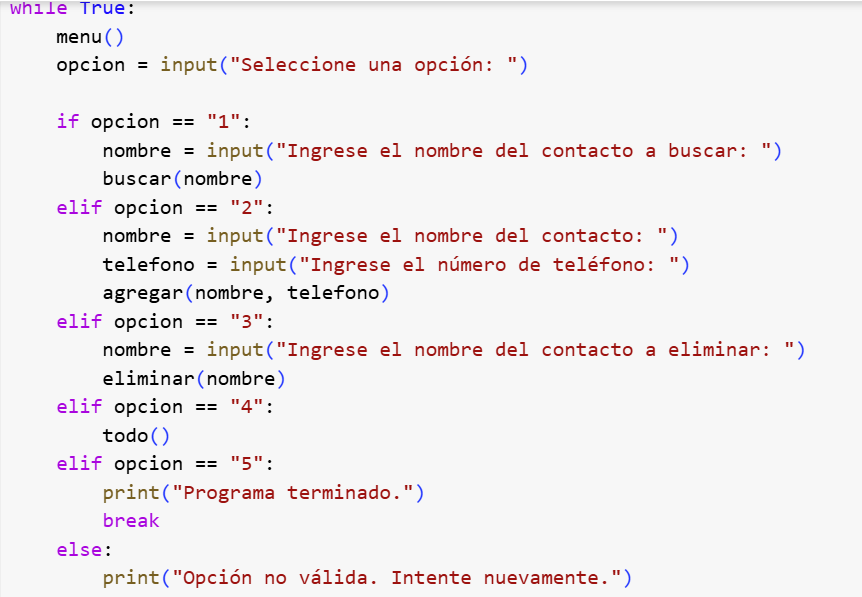
\includegraphics[width=425.2pt,height=294.5pt]{latexImage_ce1937eeb5382c952830f3382da948ff.png}}
\put(124.05,-439.92){
\includegraphics[width=187.5pt,height=33pt]{latexImage_b89161aed57e05dfe2919d781c546108.png}}
\put(124.05,-729.97){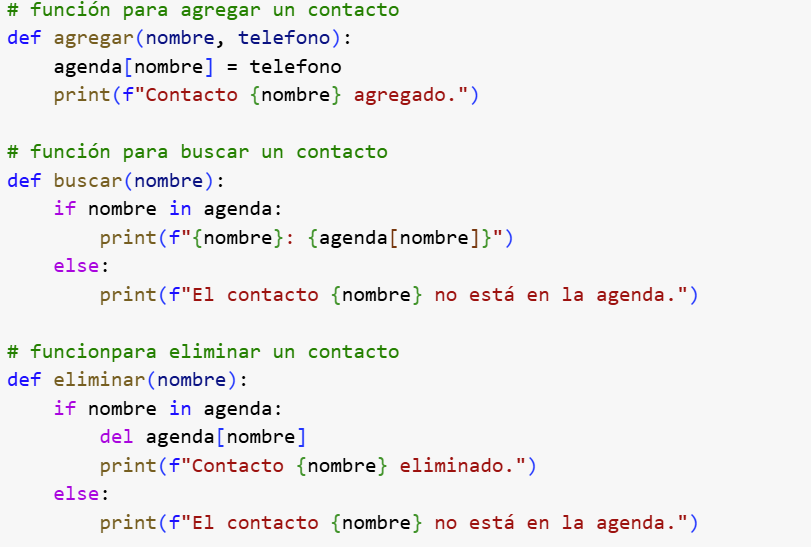
\includegraphics[width=352.2pt,height=237.55pt]{latexImage_6679f74226be95f322351ddfa8d47fa3.png}}
\end{picture}
\newpage
\begin{tikzpicture}[overlay]\path(0pt,0pt);\end{tikzpicture}
\begin{picture}(-5,0)(2.5,0)
\put(124.1,-70.20001){\fontsize{11.04}{1}\usefont{T1}{cmr}{m}{n}\selectfont\color{color_29791}Ejercicio 5:(Clases) }
\put(124.1,-84.85999){\fontsize{11.04}{1}\usefont{T1}{cmr}{m}{n}\selectfont\color{color_29791} }
\put(124.1,-100.22){\fontsize{12}{1}\usefont{T1}{cmr}{m}{n}\selectfont\color{color_29791}Primero definimos la clase con los atributos de nombre y edad }
\put(124.1,-115.22){\fontsize{11.04}{1}\usefont{T1}{cmr}{m}{n}\selectfont\color{color_29791} }
\put(415.15,-160.46){\fontsize{11.04}{1}\usefont{T1}{cmr}{m}{n}\selectfont\color{color_29791} }
\put(124.1,-172.82){\fontsize{11.04}{1}\usefont{T1}{cmr}{m}{n}\selectfont\color{color_29791} }
\put(124.1,-188.18){\fontsize{12}{1}\usefont{T1}{cmr}{m}{n}\selectfont\color{color_29791}Luego con self almacenamos los atributos }
\put(124.1,-205.1){\fontsize{12.96}{1}\usefont{T1}{cmr}{m}{n}\selectfont\color{color_29791} }
\put(295.13,-233.66){\fontsize{12.96}{1}\usefont{T1}{cmr}{m}{n}\selectfont\color{color_29791} }
\put(124.1,-245.42){\fontsize{9.96}{1}\usefont{T1}{cmr}{m}{n}\selectfont\color{color_29791} }
\put(124.1,-260.45){\fontsize{12}{1}\usefont{T1}{cmr}{m}{n}\selectfont\color{color_29791}Luego creamos un método para imprimir los datos }
\put(124.1,-277.37){\fontsize{12.96}{1}\usefont{T1}{cmr}{m}{n}\selectfont\color{color_29791} }
\put(497.62,-333.41){\fontsize{11.04}{1}\usefont{T1}{cmr}{m}{n}\selectfont\color{color_29791} }
\put(124.1,-345.65){\fontsize{11.04}{1}\usefont{T1}{cmr}{m}{n}\selectfont\color{color_29791} }
\put(106.1,-361.97){\fontsize{12}{1}\usefont{T1}{cmr}{m}{n}\selectfont\color{color_29791}• Parte2 }
\put(124.1,-377.69){\fontsize{12}{1}\usefont{T1}{cmr}{m}{n}\selectfont\color{color_29791}Primero definimos las funciones que va a hacer nuestra calculadora como }
\put(124.1,-393.65){\fontsize{12}{1}\usefont{T1}{cmr}{m}{n}\selectfont\color{color_29791}suma, resta multiplicación, división, para que estas funciones puedan operar }
\put(124.1,-409.49){\fontsize{12}{1}\usefont{T1}{cmr}{m}{n}\selectfont\color{color_29791}varios números a la vez le pasamos el argumento *args }
\put(325.63,-606.19){\fontsize{11.04}{1}\usefont{T1}{cmr}{m}{n}\selectfont\color{color_29791} }
\put(124.1,-618.46){\fontsize{11.04}{1}\usefont{T1}{cmr}{m}{n}\selectfont\color{color_29791} }
\put(124.1,-632.98){\fontsize{11.04}{1}\usefont{T1}{cmr}{m}{n}\selectfont\color{color_29791} }
\put(124.1,-648.34){\fontsize{12}{1}\usefont{T1}{cmr}{m}{n}\selectfont\color{color_29791}Luego creamos un bucle while, para que las opciones del menú se sigan }
\put(124.1,-664.18){\fontsize{12}{1}\usefont{T1}{cmr}{m}{n}\selectfont\color{color_29791}repitiendo hasta que el usuario decida salir, también imprimimos un menú }
\put(124.1,-680.14){\fontsize{12}{1}\usefont{T1}{cmr}{m}{n}\selectfont\color{color_29791}con todas las operaciones. }
\put(124.1,-695.14){\fontsize{11.04}{1}\usefont{T1}{cmr}{m}{n}\selectfont\color{color_29791} }
\put(124.05,-160.44){
\includegraphics[width=291pt,height=41pt]{latexImage_4fd0a7e7cbc285c8cc99cd59d136e27b.png}}
\put(124.05,-233.62){
\includegraphics[width=171pt,height=22.5pt]{latexImage_599171b151ca00ca69daa22ccceef698.png}}
\put(124.05,-333.34){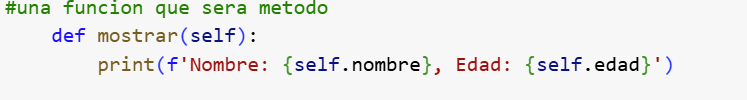
\includegraphics[width=373.5pt,height=50pt]{latexImage_79ec60c7101b0f9a06e6b9928c502ca1.png}}
\put(124.05,-606.12){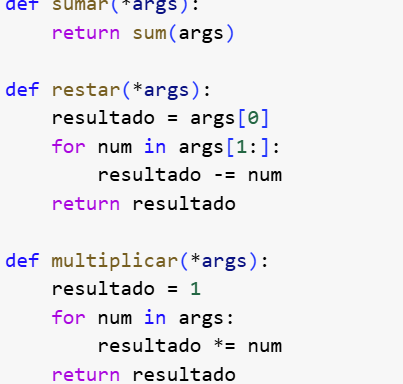
\includegraphics[width=201.5pt,height=192pt]{latexImage_4ef1aea6eaff39545361b893d036b2a9.png}}
\end{picture}
\newpage
\begin{tikzpicture}[overlay]\path(0pt,0pt);\end{tikzpicture}
\begin{picture}(-5,0)(2.5,0)
\put(472.66,-217.46){\fontsize{11.04}{1}\usefont{T1}{cmr}{m}{n}\selectfont\color{color_29791} }
\put(124.1,-229.82){\fontsize{11.04}{1}\usefont{T1}{cmr}{m}{n}\selectfont\color{color_29791} }
\put(124.1,-245.18){\fontsize{12}{1}\usefont{T1}{cmr}{m}{n}\selectfont\color{color_29791}También utilizamos if else, para ejecutar una operación según elija el }
\put(124.1,-261.05){\fontsize{12}{1}\usefont{T1}{cmr}{m}{n}\selectfont\color{color_29791}usuario. En caso de elegir “5” se termina el bucle y finaliza el programa. }
\put(124.1,-276.05){\fontsize{11.04}{1}\usefont{T1}{cmr}{m}{n}\selectfont\color{color_29791} }
\put(517.66,-454.99){\fontsize{11.04}{1}\usefont{T1}{cmr}{m}{n}\selectfont\color{color_29791}                                                                                                                       }
\put(70.104,-475.15){\fontsize{11.04}{1}\usefont{T1}{cmr}{m}{n}\selectfont\color{color_29791} }
\put(106.1,-498.43){\fontsize{11.04}{1}\usefont{T1}{cmr}{m}{n}\selectfont\color{color_29791}• Parte3(Análisis de datos con Pandas): }
\put(105.5,-521.95){\fontsize{12}{1}\usefont{T1}{cmr}{m}{n}\selectfont\color{color_29791}Estos códigos están destinados a crear un mapa utilizando datos geoespaciales y }
\put(105.5,-537.79){\fontsize{12}{1}\usefont{T1}{cmr}{m}{n}\selectfont\color{color_29791}datos de población por regiones en Perú:  }
\put(105.5,-561.67){\fontsize{12}{1}\usefont{T1}{cmr}{m}{n}\selectfont\color{color_29791}Instalación de paquetes:  }
\put(106.1,-585.55){\fontsize{12}{1}\usefont{T1}{cmr}{m}{n}\selectfont\color{color_29791}Aquí se están instalando las bibliotecas necesarias. }
\put(106.1,-601.39){\fontsize{12}{1}\usefont{T1}{cmr}{m}{n}\selectfont\color{color_29791}Geopandas: Para manejar datos geoespaciales. }
\put(106.1,-617.26){\fontsize{12}{1}\usefont{T1}{cmr}{m}{n}\selectfont\color{color_29791}Matplotlib: Para trazar gráficos. }
\put(106.1,-633.1){\fontsize{12}{1}\usefont{T1}{cmr}{m}{n}\selectfont\color{color_29791}Pandas: Para análisis de datos.}
\put(379.87,-721.18){\fontsize{11.04}{1}\usefont{T1}{cmr}{m}{n}\selectfont\color{color_29791} }
\put(124.1,-733.416){\fontsize{11.04}{1}\usefont{T1}{cmr}{m}{n}\selectfont\color{color_29791} }
\put(105.5,-756.816){\fontsize{11.04}{1}\usefont{T1}{cmr}{b}{n}\selectfont\color{color_29791}Impo}
\put(124.05,-217.43){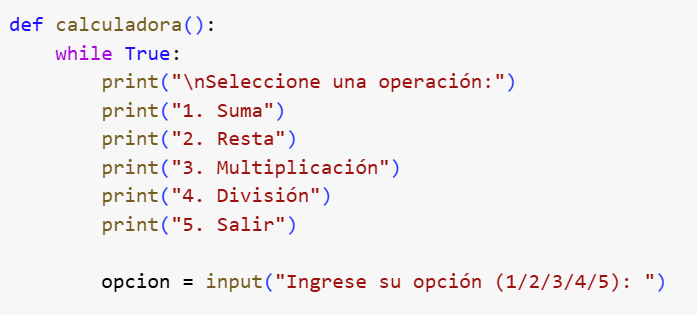
\includegraphics[width=348.5pt,height=157.5pt]{latexImage_3b26988c24a704148c7c8d450d5a4fc7.png}}
\put(124.05,-454.77){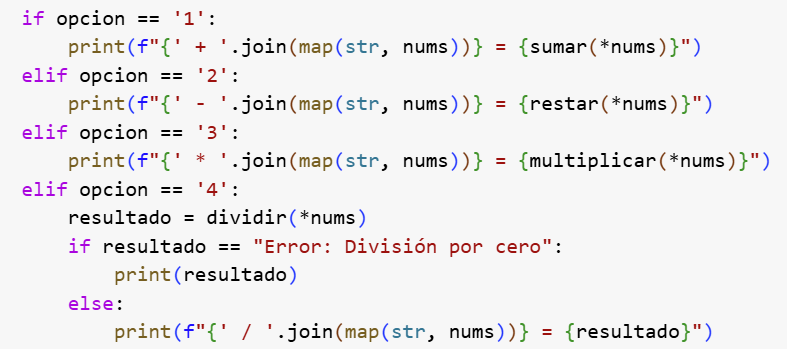
\includegraphics[width=393.5pt,height=174.5pt]{latexImage_9218eb39e64aaf3eb7689e311fc94999.png}}
\put(106.05,-721){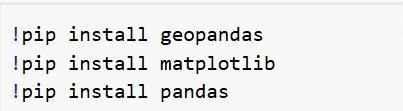
\includegraphics[width=273.75pt,height=83.25pt]{latexImage_51cdbf64977226b7c60cd9fcf3aaa4b3.png}}
\end{picture}
\newpage
\begin{tikzpicture}[overlay]\path(0pt,0pt);\end{tikzpicture}
\begin{picture}(-5,0)(2.5,0)
\put(105.5,-70.20001){\fontsize{11.04}{1}\usefont{T1}{cmr}{m}{n}\selectfont\color{color_29791}Se importan todas las bibliotecas necesarias para trabajar con datos geoespaciales( }
\put(105.5,-85.70001){\fontsize{11.04}{1}\usefont{T1}{cmr}{m}{n}\selectfont\color{color_29791}geopandas, cartopy), manipulación de datos (pandas, numpy) y }
\put(105.5,-100.22){\fontsize{11.04}{1}\usefont{T1}{cmr}{m}{n}\selectfont\color{color_29791}visualización(matplotlib).}
\put(434.02,-317.33){\fontsize{11.04}{1}\usefont{T1}{cmr}{m}{n}\selectfont\color{color_29791} }
\put(124.1,-337.61){\fontsize{11.04}{1}\usefont{T1}{cmr}{m}{n}\selectfont\color{color_29791} }
\put(105.5,-361.13){\fontsize{11.04}{1}\usefont{T1}{cmr}{b}{n}\selectfont\color{color_29791}Leer datos geoespaciales del Perú: }
\put(105.5,-384.53){\fontsize{11.04}{1}\usefont{T1}{cmr}{m}{n}\selectfont\color{color_29791}Lee un archivo GeoJSON (peru\_departamental\_simple.geojson) que contiene }
\put(105.5,-400.01){\fontsize{11.04}{1}\usefont{T1}{cmr}{m}{n}\selectfont\color{color_29791}los límites geoespaciales de las regiones departamentales del Perú. }
\put(511.3,-485.11){\fontsize{11.04}{1}\usefont{T1}{cmr}{m}{n}\selectfont\color{color_29791} }
\put(511.3,-618.94){\fontsize{11.04}{1}\usefont{T1}{cmr}{m}{n}\selectfont\color{color_29791} }
\put(105.5,-640.06){\fontsize{12}{1}\usefont{T1}{cmr}{m}{n}\selectfont\color{color_29791}Leer datos de población por regiones: }
\put(105.5,-663.94){\fontsize{12}{1}\usefont{T1}{cmr}{m}{n}\selectfont\color{color_29791}Lee un archivo de Excel (poblacion2020.xlsx) que contiene datos de }
\put(105.5,-680.26){\fontsize{12}{1}\usefont{T1}{cmr}{m}{n}\selectfont\color{color_29791}poblac}
\put(105.45,-317.24){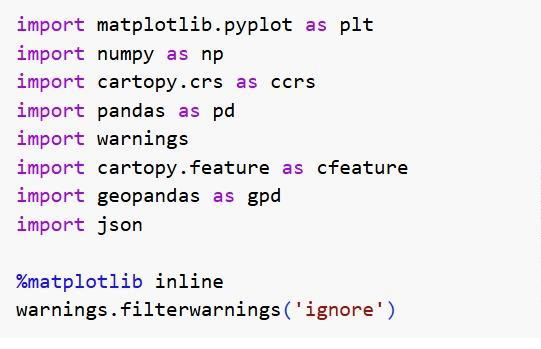
\includegraphics[width=328.45pt,height=211.88pt]{latexImage_cc48c8823dbf4f8e8a5c3b1c67faf733.png}}
\put(105.45,-485.04){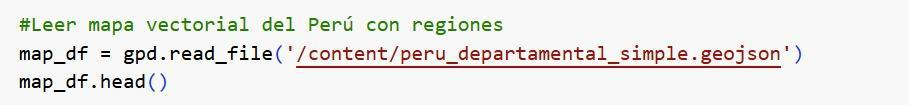
\includegraphics[width=405.75pt,height=72pt]{latexImage_2147b87119de85c59a3823313587db16.png}}
\put(105.45,-618.81){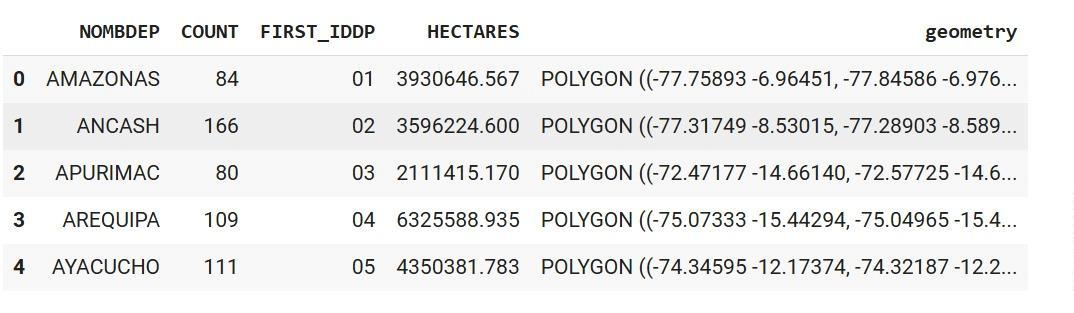
\includegraphics[width=405.75pt,height=123.75pt]{latexImage_3cd915e942b20b9c57357342ee61d0b6.png}}
\end{picture}
\newpage
\begin{tikzpicture}[overlay]\path(0pt,0pt);\end{tikzpicture}
\begin{picture}(-5,0)(2.5,0)
\put(514.3,-134.18){\fontsize{12}{1}\usefont{T1}{cmr}{m}{n}\selectfont\color{color_29791} }
\put(416.23,-603.31){\fontsize{11.04}{1}\usefont{T1}{cmr}{m}{n}\selectfont\color{color_29791} }
\put(70.104,-623.62){\fontsize{11.04}{1}\usefont{T1}{cmr}{m}{n}\selectfont\color{color_29791} }
\put(124.1,-646.18){\fontsize{11.04}{1}\usefont{T1}{cmr}{m}{n}\selectfont\color{color_29791} }
\put(105.5,-669.58){\fontsize{12}{1}\usefont{T1}{cmr}{m}{n}\selectfont\color{color_29791}Unir DataFrames: }
\put(105.5,-693.46){\fontsize{12}{1}\usefont{T1}{cmr}{m}{n}\selectfont\color{color_29791}Une los dos DataFrames (map\_df y data\_df) utilizando la columna NOMBDEP }
\put(105.5,-709.9){\fontsize{12}{1}\usefont{T1}{cmr}{m}{n}\selectfont\color{color_29791}de map\_df y DEPARTAMENTO de data\_df. }
\put(105.5,-732.936){\fontsize{11.04}{1}\usefont{T1}{cmr}{m}{n}\selectfont\color{color_29791} }
\put(105.45,-134.18){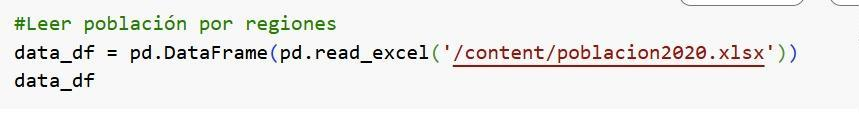
\includegraphics[width=408.75pt,height=74.25pt]{latexImage_4ca7613cc2640a548634bb512da31afd.png}}
\put(184.47,-603.1899){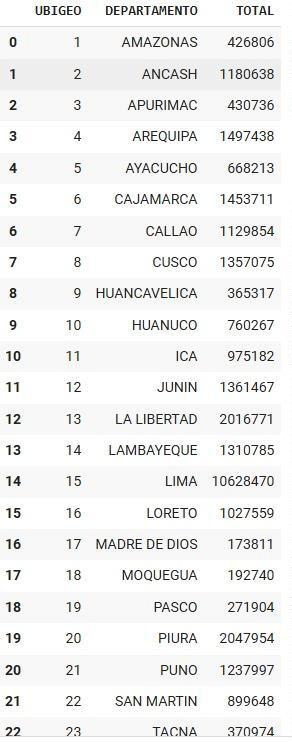
\includegraphics[width=231.75pt,height=459pt]{latexImage_87dda677bf93cb1a5e49f8f7995975b9.png}}
\end{picture}
\newpage
\begin{tikzpicture}[overlay]\path(0pt,0pt);\end{tikzpicture}
\begin{picture}(-5,0)(2.5,0)
\put(501.58,-118.46){\fontsize{11.04}{1}\usefont{T1}{cmr}{m}{n}\selectfont\color{color_29791} }
\put(530.74,-245.42){\fontsize{11.04}{1}\usefont{T1}{cmr}{m}{n}\selectfont\color{color_29791} }
\put(105.5,-265.85){\fontsize{11.04}{1}\usefont{T1}{cmr}{m}{n}\selectfont\color{color_29791} }
\put(105.5,-289.25){\fontsize{12}{1}\usefont{T1}{cmr}{m}{n}\selectfont\color{color_29791}Selección de columnas de interés:  }
\put(105.5,-313.13){\fontsize{12}{1}\usefont{T1}{cmr}{m}{n}\selectfont\color{color_29791}Selecciona las columnas relevantes para el análisis (DEPARTAMENTO, TOTAL de }
\put(105.5,-329.57){\fontsize{12}{1}\usefont{T1}{cmr}{m}{n}\selectfont\color{color_29791}población y geometry para los límites geoespaciales). }
\put(518.02,-407.81){\fontsize{11.04}{1}\usefont{T1}{cmr}{m}{n}\selectfont\color{color_29791} }
\put(423.46,-632.5){\fontsize{11.04}{1}\usefont{T1}{cmr}{m}{n}\selectfont\color{color_29791} }
\put(282.65,-652.66){\fontsize{11.04}{1}\usefont{T1}{cmr}{m}{n}\selectfont\color{color_29791} }
\put(105.5,-675.22){\fontsize{11.04}{1}\usefont{T1}{cmr}{m}{n}\selectfont\color{color_29791} }
\put(105.5,-697.78){\fontsize{11.04}{1}\usefont{T1}{cmr}{m}{n}\selectfont\color{color_29791} }
\put(105.45,-118.43){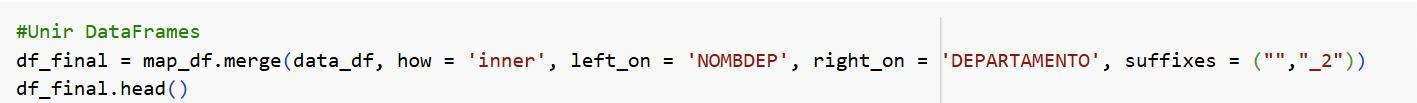
\includegraphics[width=396pt,height=58.5pt]{latexImage_d41d550d94a3a517fe4ddbc988f5c254.png}}
\put(105.45,-245.44){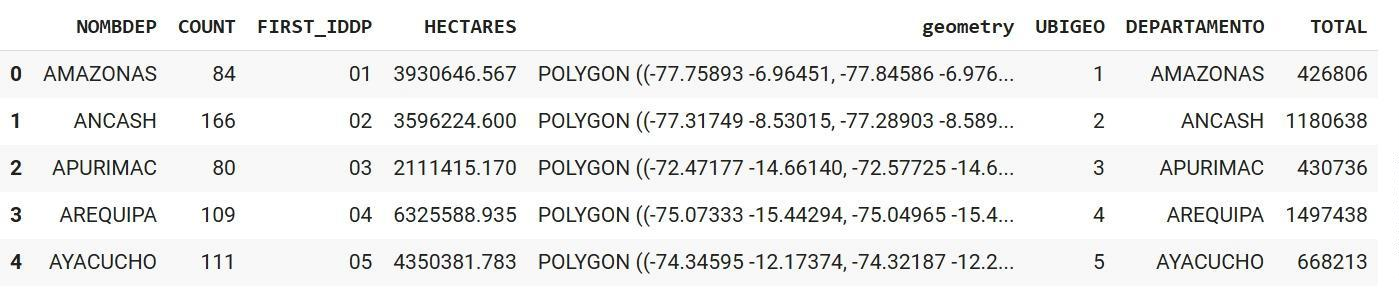
\includegraphics[width=425.25pt,height=117pt]{latexImage_23d5fe1544950e65978a70ee33f7c992.png}}
\put(105.45,-407.76){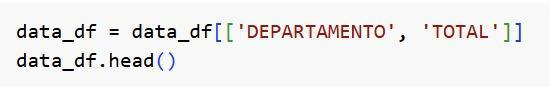
\includegraphics[width=412.45pt,height=65.242pt]{latexImage_2781eb4cd0cd4bedf00b593bb45cfca9.png}}
\put(177.35,-632.28){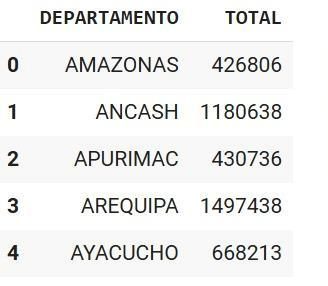
\includegraphics[width=246pt,height=214.5pt]{latexImage_a116530a3bcffc0fa26882993eb9f346.png}}
\end{picture}
\newpage
\begin{tikzpicture}[overlay]\path(0pt,0pt);\end{tikzpicture}
\begin{picture}(-5,0)(2.5,0)
\put(530.74,-119.9){\fontsize{11.04}{1}\usefont{T1}{cmr}{m}{n}\selectfont\color{color_29791} }
\put(105.5,-140.3){\fontsize{11.04}{1}\usefont{T1}{cmr}{m}{n}\selectfont\color{color_29791} }
\put(105.5,-162.86){\fontsize{11.04}{1}\usefont{T1}{cmr}{m}{n}\selectfont\color{color_29791} }
\put(105.5,-185.42){\fontsize{11.04}{1}\usefont{T1}{cmr}{m}{n}\selectfont\color{color_29791}Visualización del mapa:  }
\put(105.5,-208.94){\fontsize{12}{1}\usefont{T1}{cmr}{m}{n}\selectfont\color{color_29791}Finalmente, traza el mapa utilizando los datos combinados (df\_final). }
\put(105.5,-233.06){\fontsize{12}{1}\usefont{T1}{cmr}{m}{n}\selectfont\color{color_29791}Este proceso combina datos geoespaciales con datos numéricos (en este caso, }
\put(105.5,-248.9){\fontsize{12}{1}\usefont{T1}{cmr}{m}{n}\selectfont\color{color_29791}población) para crear un mapa temático que muestra la distribución de la }
\put(105.5,-264.89){\fontsize{12}{1}\usefont{T1}{cmr}{m}{n}\selectfont\color{color_29791}población en los departamentos de Perú }
\put(458.26,-668.5){\fontsize{11.04}{1}\usefont{T1}{cmr}{m}{n}\selectfont\color{color_29791} }
\put(105.5,-688.66){\fontsize{11.04}{1}\usefont{T1}{cmr}{m}{n}\selectfont\color{color_29791}´ }
\put(105.5,-711.22){\fontsize{11.04}{1}\usefont{T1}{cmr}{m}{n}\selectfont\color{color_29791} }
\put(88.1,-740.256){\fontsize{18}{1}\usefont{T1}{cmr}{m}{n}\selectfont\color{color_29791}4.}
\put(105.45,-119.93){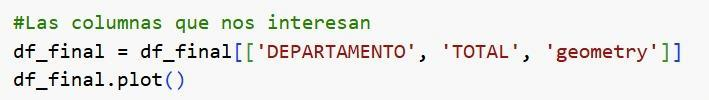
\includegraphics[width=425.25pt,height=60pt]{latexImage_5897a6cc63a6faf12e0b43f863dda0e2.png}}
\put(142.47,-668.26){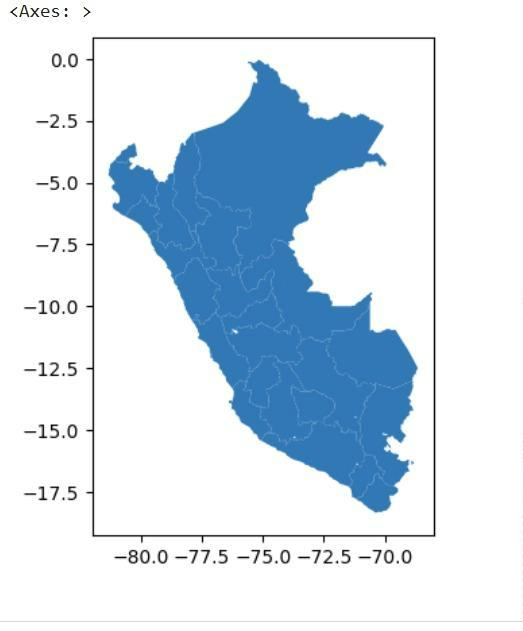
\includegraphics[width=315.75pt,height=390.75pt]{latexImage_6dd0e426187f1ce21df0f810eccc834f.png}}
\end{picture}
\newpage
\begin{tikzpicture}[overlay]\path(0pt,0pt);\end{tikzpicture}
\begin{picture}(-5,0)(2.5,0)
\put(70.104,-71.03998){\fontsize{12}{1}\usefont{T1}{cmr}{m}{n}\selectfont\color{color_29791}Python permite interactuar al usuario de forma sencilla, también es fácil integrar los }
\put(70.104,-87.02002){\fontsize{12}{1}\usefont{T1}{cmr}{m}{n}\selectfont\color{color_29791}datos, con bibliotecas como mathplotlib y cartopy. }
\end{picture}
\end{document}